\documentclass[1p]{elsarticle_modified}
%\bibliographystyle{elsarticle-num}

%\usepackage[colorlinks]{hyperref}
%\usepackage{abbrmath_seonhwa} %\Abb, \Ascr, \Acal ,\Abf, \Afrak
\usepackage{amsfonts}
\usepackage{amssymb}
\usepackage{amsmath}
\usepackage{amsthm}
\usepackage{scalefnt}
\usepackage{amsbsy}
\usepackage{kotex}
\usepackage{caption}
\usepackage{subfig}
\usepackage{color}
\usepackage{graphicx}
\usepackage{xcolor} %% white, black, red, green, blue, cyan, magenta, yellow
\usepackage{float}
\usepackage{setspace}
\usepackage{hyperref}

\usepackage{tikz}
\usetikzlibrary{arrows}

\usepackage{multirow}
\usepackage{array} % fixed length table
\usepackage{hhline}

%%%%%%%%%%%%%%%%%%%%%
\makeatletter
\renewcommand*\env@matrix[1][\arraystretch]{%
	\edef\arraystretch{#1}%
	\hskip -\arraycolsep
	\let\@ifnextchar\new@ifnextchar
	\array{*\c@MaxMatrixCols c}}
\makeatother %https://tex.stackexchange.com/questions/14071/how-can-i-increase-the-line-spacing-in-a-matrix
%%%%%%%%%%%%%%%

\usepackage[normalem]{ulem}

\newcommand{\msout}[1]{\ifmmode\text{\sout{\ensuremath{#1}}}\else\sout{#1}\fi}
%SOURCE: \msout is \stkout macro in https://tex.stackexchange.com/questions/20609/strikeout-in-math-mode

\newcommand{\cancel}[1]{
	\ifmmode
	{\color{red}\msout{#1}}
	\else
	{\color{red}\sout{#1}}
	\fi
}

\newcommand{\add}[1]{
	{\color{blue}\uwave{#1}}
}

\newcommand{\replace}[2]{
	\ifmmode
	{\color{red}\msout{#1}}{\color{blue}\uwave{#2}}
	\else
	{\color{red}\sout{#1}}{\color{blue}\uwave{#2}}
	\fi
}

\newcommand{\Sol}{\mathcal{S}} %segment
\newcommand{\D}{D} %diagram
\newcommand{\A}{\mathcal{A}} %arc


%%%%%%%%%%%%%%%%%%%%%%%%%%%%%5 test

\def\sl{\operatorname{\textup{SL}}(2,\Cbb)}
\def\psl{\operatorname{\textup{PSL}}(2,\Cbb)}
\def\quan{\mkern 1mu \triangleright \mkern 1mu}

\theoremstyle{definition}
\newtheorem{thm}{Theorem}[section]
\newtheorem{prop}[thm]{Proposition}
\newtheorem{lem}[thm]{Lemma}
\newtheorem{ques}[thm]{Question}
\newtheorem{cor}[thm]{Corollary}
\newtheorem{defn}[thm]{Definition}
\newtheorem{exam}[thm]{Example}
\newtheorem{rmk}[thm]{Remark}
\newtheorem{alg}[thm]{Algorithm}

\newcommand{\I}{\sqrt{-1}}
\begin{document}

%\begin{frontmatter}
%
%\title{Boundary parabolic representations of knots up to 8 crossings}
%
%%% Group authors per affiliation:
%\author{Yunhi Cho} 
%\address{Department of Mathematics, University of Seoul, Seoul, Korea}
%\ead{yhcho@uos.ac.kr}
%
%
%\author{Seonhwa Kim} %\fnref{s_kim}}
%\address{Center for Geometry and Physics, Institute for Basic Science, Pohang, 37673, Korea}
%\ead{ryeona17@ibs.re.kr}
%
%\author{Hyuk Kim}
%\address{Department of Mathematical Sciences, Seoul National University, Seoul 08826, Korea}
%\ead{hyukkim@snu.ac.kr}
%
%\author{Seokbeom Yoon}
%\address{Department of Mathematical Sciences, Seoul National University, Seoul, 08826,  Korea}
%\ead{sbyoon15@snu.ac.kr}
%
%\begin{abstract}
%We find all boundary parabolic representation of knots up to 8 crossings.
%
%\end{abstract}
%\begin{keyword}
%    \MSC[2010] 57M25 
%\end{keyword}
%
%\end{frontmatter}

%\linenumbers
%\tableofcontents
%
\newcommand\colored[1]{\textcolor{white}{\rule[-0.35ex]{0.8em}{1.4ex}}\kern-0.8em\color{red} #1}%
%\newcommand\colored[1]{\textcolor{white}{ #1}\kern-2.17ex	\textcolor{white}{ #1}\kern-1.81ex	\textcolor{white}{ #1}\kern-2.15ex\color{red}#1	}

{\Large $\underline{11a_{215}~(K11a_{215})}$}

\setlength{\tabcolsep}{10pt}
\renewcommand{\arraystretch}{1.6}
\vspace{1cm}\begin{tabular}{m{100pt}>{\centering\arraybackslash}m{274pt}}
\multirow{5}{120pt}{
	\centering
	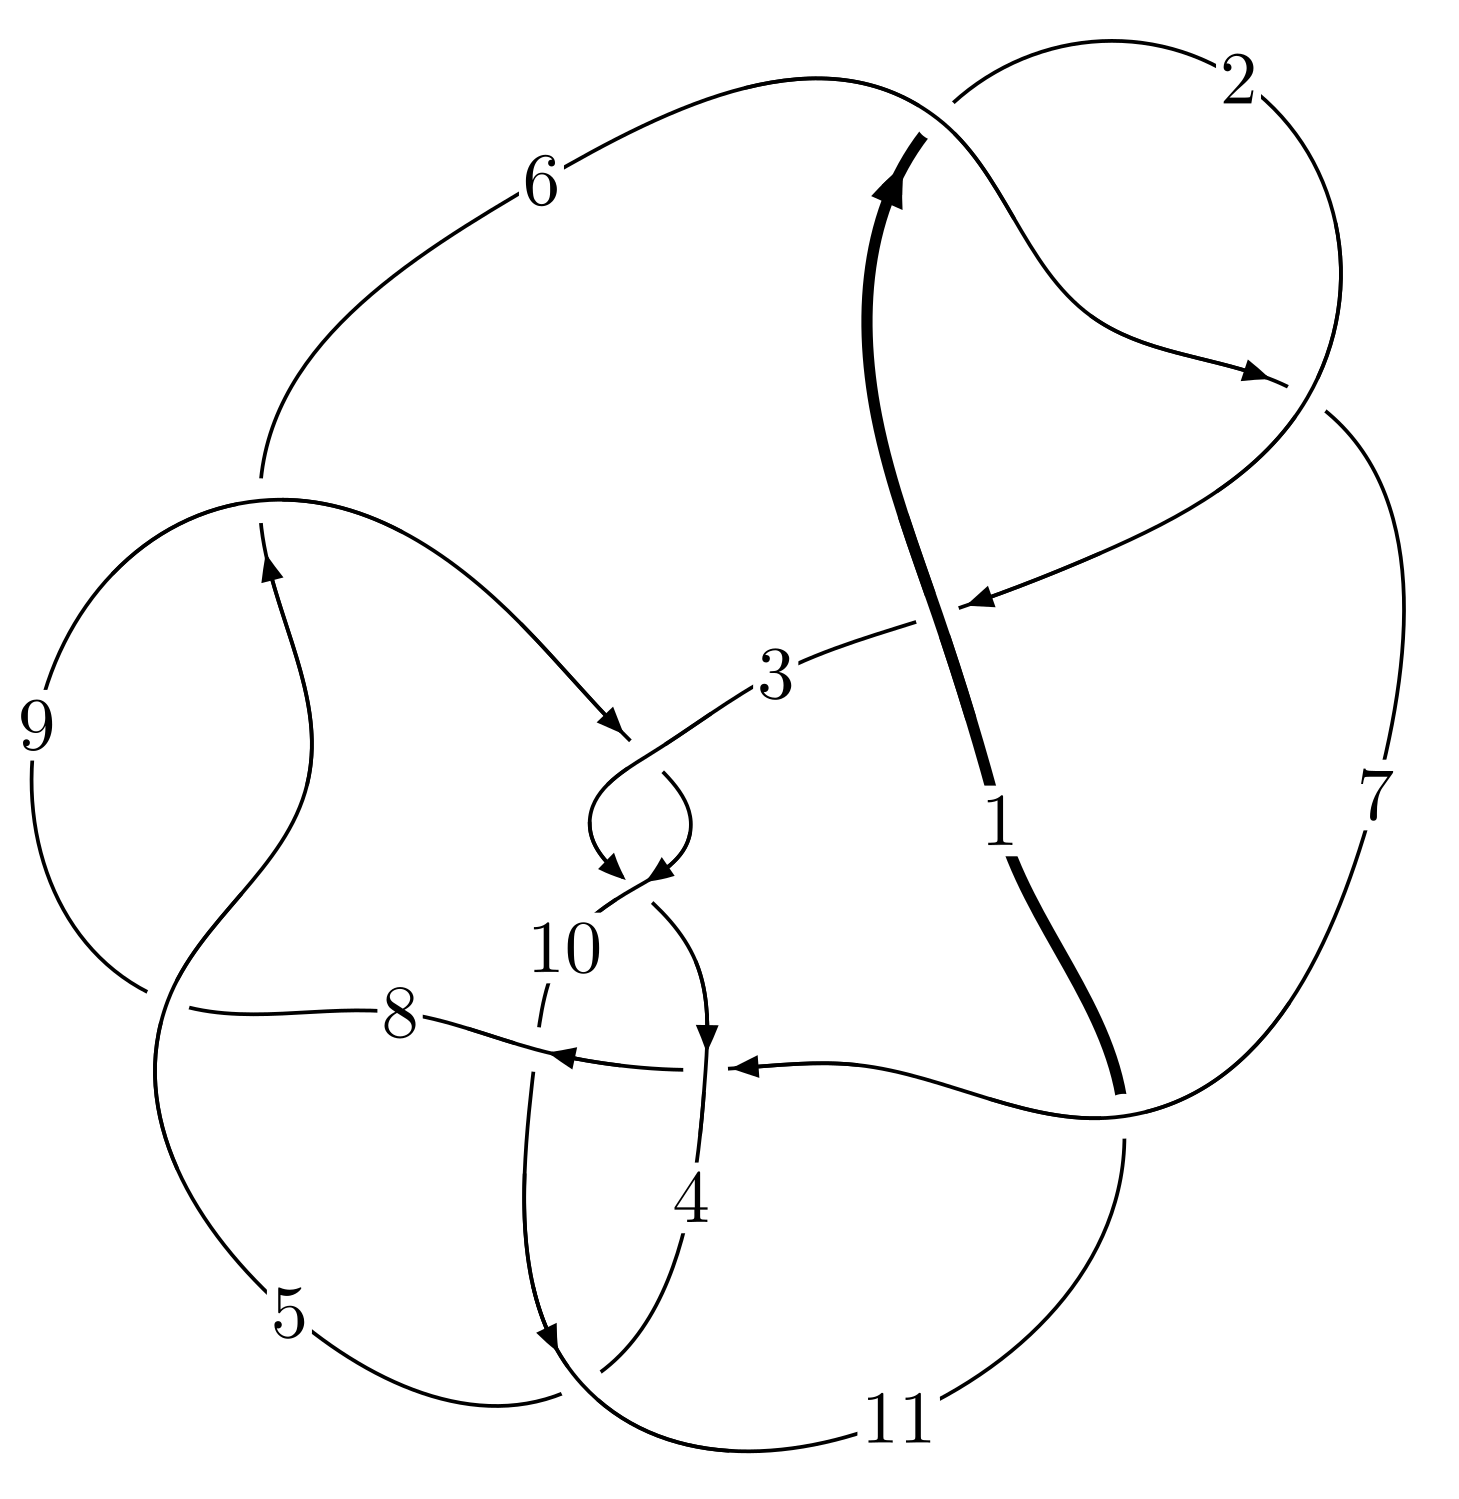
\includegraphics[width=112pt]{../../../GIT/diagram.site/Diagrams/png/464_11a_215.png}\\
\ \ \ A knot diagram\footnotemark}&
\allowdisplaybreaks
\textbf{Linearized knot diagam} \\
\cline{2-2}
 &
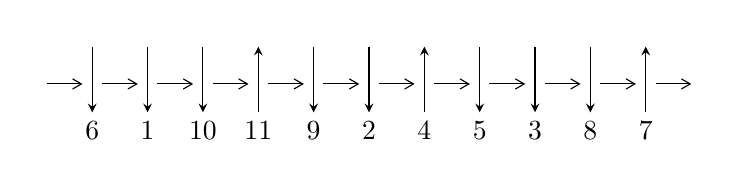
\begin{tikzpicture}[x=20pt, y=17pt]
	% nodes
	\node (C0) at (0, 0) {};
	\node (C1) at (1, 0) {};
	\node (C1U) at (1, +1) {};
	\node (C1D) at (1, -1) {6};

	\node (C2) at (2, 0) {};
	\node (C2U) at (2, +1) {};
	\node (C2D) at (2, -1) {1};

	\node (C3) at (3, 0) {};
	\node (C3U) at (3, +1) {};
	\node (C3D) at (3, -1) {10};

	\node (C4) at (4, 0) {};
	\node (C4U) at (4, +1) {};
	\node (C4D) at (4, -1) {11};

	\node (C5) at (5, 0) {};
	\node (C5U) at (5, +1) {};
	\node (C5D) at (5, -1) {9};

	\node (C6) at (6, 0) {};
	\node (C6U) at (6, +1) {};
	\node (C6D) at (6, -1) {2};

	\node (C7) at (7, 0) {};
	\node (C7U) at (7, +1) {};
	\node (C7D) at (7, -1) {4};

	\node (C8) at (8, 0) {};
	\node (C8U) at (8, +1) {};
	\node (C8D) at (8, -1) {5};

	\node (C9) at (9, 0) {};
	\node (C9U) at (9, +1) {};
	\node (C9D) at (9, -1) {3};

	\node (C10) at (10, 0) {};
	\node (C10U) at (10, +1) {};
	\node (C10D) at (10, -1) {8};

	\node (C11) at (11, 0) {};
	\node (C11U) at (11, +1) {};
	\node (C11D) at (11, -1) {7};
	\node (C12) at (12, 0) {};

	% arrows
	\draw[->,>={angle 60}]
	(C0) edge (C1) (C1) edge (C2) (C2) edge (C3) (C3) edge (C4) (C4) edge (C5) (C5) edge (C6) (C6) edge (C7) (C7) edge (C8) (C8) edge (C9) (C9) edge (C10) (C10) edge (C11) (C11) edge (C12) ;	\draw[->,>=stealth]
	(C1U) edge (C1D) (C2U) edge (C2D) (C3U) edge (C3D) (C4D) edge (C4U) (C5U) edge (C5D) (C6U) edge (C6D) (C7D) edge (C7U) (C8U) edge (C8D) (C9U) edge (C9D) (C10U) edge (C10D) (C11D) edge (C11U) ;
	\end{tikzpicture} \\
\hhline{~~} \\& 
\textbf{Solving Sequence} \\ \cline{2-2} 
 &
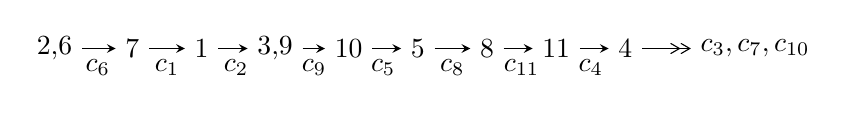
\begin{tikzpicture}[x=25pt, y=7pt]
	% node
	\node (A0) at (-1/8, 0) {2,6};
	\node (A1) at (1, 0) {7};
	\node (A2) at (2, 0) {1};
	\node (A3) at (49/16, 0) {3,9};
	\node (A4) at (33/8, 0) {10};
	\node (A5) at (41/8, 0) {5};
	\node (A6) at (49/8, 0) {8};
	\node (A7) at (57/8, 0) {11};
	\node (A8) at (65/8, 0) {4};
	\node (C1) at (1/2, -1) {$c_{6}$};
	\node (C2) at (3/2, -1) {$c_{1}$};
	\node (C3) at (5/2, -1) {$c_{2}$};
	\node (C4) at (29/8, -1) {$c_{9}$};
	\node (C5) at (37/8, -1) {$c_{5}$};
	\node (C6) at (45/8, -1) {$c_{8}$};
	\node (C7) at (53/8, -1) {$c_{11}$};
	\node (C8) at (61/8, -1) {$c_{4}$};
	\node (A9) at (10, 0) {$c_{3},c_{7},c_{10}$};

	% edge
	\draw[->,>=stealth]	
	(A0) edge (A1) (A1) edge (A2) (A2) edge (A3) (A3) edge (A4) (A4) edge (A5) (A5) edge (A6) (A6) edge (A7) (A7) edge (A8) ;
	\draw[->>,>={angle 60}]	
	(A8) edge (A9);
\end{tikzpicture} \\ 

\end{tabular} \\

\footnotetext{
The image of knot diagram is generated by the software ``\textbf{Draw programme}" developed by Andrew Bartholomew(\url{http://www.layer8.co.uk/maths/draw/index.htm\#Running-draw}), where we modified some parts for our purpose(\url{https://github.com/CATsTAILs/LinksPainter}).
}\phantom \\ \newline 
\centering \textbf{Ideals for irreducible components\footnotemark of $X_{\text{par}}$} 
 
\begin{align*}
I^u_{1}&=\langle 
-29 u^{26}+175 u^{25}+\cdots+4 b+156,\;-41 u^{26}+209 u^{25}+\cdots+8 a+92,\;u^{27}-7 u^{26}+\cdots-48 u+8\rangle \\
I^u_{2}&=\langle 
-4.28042\times10^{21} a^{5} u^{8}+3.83114\times10^{22} a^{4} u^{8}+\cdots-6.06064\times10^{22} a+4.42208\times10^{22},\\
\phantom{I^u_{2}}&\phantom{= \langle  }3 u^8 a^3+9 u^8 a^2+\cdots-18 a-43,\;u^9+u^8-2 u^7-3 u^6+u^5+3 u^4+2 u^3- u-1\rangle \\
I^u_{3}&=\langle 
- u^{14}+3 u^{12}-5 u^{10}+3 u^8+u^7- u^6-2 u^5- u^4+2 u^3+b- u-1,\\
\phantom{I^u_{3}}&\phantom{= \langle  }u^{14}-3 u^{13}-3 u^{12}+10 u^{11}+4 u^{10}-17 u^9- u^8+11 u^7+u^6- u^5-6 u^4-3 u^3+8 u^2+a- u-4,\\
\phantom{I^u_{3}}&\phantom{= \langle  }u^{15}-4 u^{13}+8 u^{11}-8 u^9- u^8+4 u^7+3 u^6-4 u^4+3 u^2-1\rangle \\
\\
\end{align*}
\raggedright * 3 irreducible components of $\dim_{\mathbb{C}}=0$, with total 96 representations.\\
\footnotetext{All coefficients of polynomials are rational numbers. But the coefficients are sometimes approximated in decimal forms when there is not enough margin.}
\newpage
\renewcommand{\arraystretch}{1}
\centering \section*{I. $I^u_{1}= \langle -29 u^{26}+175 u^{25}+\cdots+4 b+156,\;-41 u^{26}+209 u^{25}+\cdots+8 a+92,\;u^{27}-7 u^{26}+\cdots-48 u+8 \rangle$}
\flushleft \textbf{(i) Arc colorings}\\
\begin{tabular}{m{7pt} m{180pt} m{7pt} m{180pt} }
\flushright $a_{2}=$&$\begin{pmatrix}0\\u\end{pmatrix}$ \\
\flushright $a_{6}=$&$\begin{pmatrix}1\\0\end{pmatrix}$ \\
\flushright $a_{7}=$&$\begin{pmatrix}1\\u^2\end{pmatrix}$ \\
\flushright $a_{1}=$&$\begin{pmatrix}u\\u\end{pmatrix}$ \\
\flushright $a_{3}=$&$\begin{pmatrix}- u^3\\- u^3+u\end{pmatrix}$ \\
\flushright $a_{9}=$&$\begin{pmatrix}5.12500 u^{26}-26.1250 u^{25}+\cdots+76.5000 u-11.5000\\\frac{29}{4} u^{26}-\frac{175}{4} u^{25}+\cdots+\frac{447}{2} u-39\end{pmatrix}$ \\
\flushright $a_{10}=$&$\begin{pmatrix}4.12500 u^{26}-26.1250 u^{25}+\cdots+212.500 u-43.5000\\-\frac{3}{4} u^{26}+\frac{5}{4} u^{25}+\cdots+\frac{101}{2} u-13\end{pmatrix}$ \\
\flushright $a_{5}=$&$\begin{pmatrix}6 u^{26}-\frac{67}{2} u^{25}+\cdots+128 u-\frac{39}{2}\\\frac{5}{2} u^{26}-17 u^{25}+\cdots+\frac{345}{2} u-36\end{pmatrix}$ \\
\flushright $a_{8}=$&$\begin{pmatrix}\frac{19}{4} u^{26}-\frac{53}{2} u^{25}+\cdots+\frac{321}{4} u-11\\\frac{17}{4} u^{26}-\frac{101}{4} u^{25}+\cdots+106 u-16\end{pmatrix}$ \\
\flushright $a_{11}=$&$\begin{pmatrix}u^3\\u^5- u^3+u\end{pmatrix}$ \\
\flushright $a_{4}=$&$\begin{pmatrix}-4 u^{26}+\frac{45}{2} u^{25}+\cdots-76 u+\frac{25}{2}\\\frac{3}{2} u^{25}-\frac{13}{2} u^{24}+\cdots-\frac{71}{2} u+8\end{pmatrix}$\\ \flushright $a_{4}=$&$\begin{pmatrix}-4 u^{26}+\frac{45}{2} u^{25}+\cdots-76 u+\frac{25}{2}\\\frac{3}{2} u^{25}-\frac{13}{2} u^{24}+\cdots-\frac{71}{2} u+8\end{pmatrix}$\\&\end{tabular}
\flushleft \textbf{(ii) Obstruction class $= -1$}\\~\\
\flushleft \textbf{(iii) Cusp Shapes $= 7 u^{26}-42 u^{25}+85 u^{24}+32 u^{23}-464 u^{22}+782 u^{21}+58 u^{20}-2162 u^{19}+3200 u^{18}-304 u^{17}-5341 u^{16}+7635 u^{15}-2013 u^{14}-7580 u^{13}+11422 u^{12}-4923 u^{11}-5645 u^{10}+10277 u^9-6041 u^8-1288 u^7+4988 u^6-3826 u^5+1037 u^4+557 u^3-655 u^2+276 u-46$}\\~\\
\newpage\renewcommand{\arraystretch}{1}
\flushleft \textbf{(iv) u-Polynomials at the component}\newline \\
\begin{tabular}{m{50pt}|m{274pt}}
Crossings & \hspace{64pt}u-Polynomials at each crossing \\
\hline $$\begin{aligned}c_{1},c_{6}\end{aligned}$$&$\begin{aligned}
&u^{27}-7 u^{26}+\cdots-48 u+8
\end{aligned}$\\
\hline $$\begin{aligned}c_{2}\end{aligned}$$&$\begin{aligned}
&u^{27}+13 u^{26}+\cdots+224 u+64
\end{aligned}$\\
\hline $$\begin{aligned}c_{3},c_{5},c_{8}\\c_{9}\end{aligned}$$&$\begin{aligned}
&u^{27}+u^{26}+\cdots+2 u+1
\end{aligned}$\\
\hline $$\begin{aligned}c_{4},c_{7}\end{aligned}$$&$\begin{aligned}
&u^{27}+3 u^{25}+\cdots+3 u+1
\end{aligned}$\\
\hline $$\begin{aligned}c_{10}\end{aligned}$$&$\begin{aligned}
&u^{27}-27 u^{26}+\cdots-7424 u+512
\end{aligned}$\\
\hline $$\begin{aligned}c_{11}\end{aligned}$$&$\begin{aligned}
&u^{27}-21 u^{26}+\cdots-19888 u+2664
\end{aligned}$\\
\hline
\end{tabular}\\~\\
\newpage\renewcommand{\arraystretch}{1}
\flushleft \textbf{(v) Riley Polynomials at the component}\newline \\
\begin{tabular}{m{50pt}|m{274pt}}
Crossings & \hspace{64pt}Riley Polynomials at each crossing \\
\hline $$\begin{aligned}c_{1},c_{6}\end{aligned}$$&$\begin{aligned}
&y^{27}-13 y^{26}+\cdots+224 y-64
\end{aligned}$\\
\hline $$\begin{aligned}c_{2}\end{aligned}$$&$\begin{aligned}
&y^{27}- y^{26}+\cdots+2560 y-4096
\end{aligned}$\\
\hline $$\begin{aligned}c_{3},c_{5},c_{8}\\c_{9}\end{aligned}$$&$\begin{aligned}
&y^{27}-25 y^{26}+\cdots-10 y-1
\end{aligned}$\\
\hline $$\begin{aligned}c_{4},c_{7}\end{aligned}$$&$\begin{aligned}
&y^{27}+6 y^{26}+\cdots+3 y-1
\end{aligned}$\\
\hline $$\begin{aligned}c_{10}\end{aligned}$$&$\begin{aligned}
&y^{27}-5 y^{26}+\cdots+2424832 y-262144
\end{aligned}$\\
\hline $$\begin{aligned}c_{11}\end{aligned}$$&$\begin{aligned}
&y^{27}+15 y^{26}+\cdots+24224224 y-7096896
\end{aligned}$\\
\hline
\end{tabular}\\~\\
\newpage\flushleft \textbf{(vi) Complex Volumes and Cusp Shapes}
$$\begin{array}{c|c|c}  
\text{Solutions to }I^u_{1}& \I (\text{vol} + \sqrt{-1}CS) & \text{Cusp shape}\\
 \hline 
\begin{aligned}
u &= \phantom{-}0.250449 + 1.038140 I \\
a &= -0.444857 - 0.280509 I \\
b &= -1.222090 + 0.179844 I\end{aligned}
 & -5.84917 + 1.93910 I & -18.8822 - 3.3310 I \\ \hline\begin{aligned}
u &= \phantom{-}0.250449 - 1.038140 I \\
a &= -0.444857 + 0.280509 I \\
b &= -1.222090 - 0.179844 I\end{aligned}
 & -5.84917 - 1.93910 I & -18.8822 + 3.3310 I \\ \hline\begin{aligned}
u &= \phantom{-}0.942577 + 0.503851 I \\
a &= -0.932522 + 0.762632 I \\
b &= -0.482241 - 0.629621 I\end{aligned}
 & \phantom{-}1.12638 - 3.49850 I & -2.08740 + 6.42119 I \\ \hline\begin{aligned}
u &= \phantom{-}0.942577 - 0.503851 I \\
a &= -0.932522 - 0.762632 I \\
b &= -0.482241 + 0.629621 I\end{aligned}
 & \phantom{-}1.12638 + 3.49850 I & -2.08740 - 6.42119 I \\ \hline\begin{aligned}
u &= \phantom{-}0.206067 + 0.899919 I \\
a &= \phantom{-}0.523648 + 0.537105 I \\
b &= \phantom{-}1.48683 - 0.50104 I\end{aligned}
 & -8.00804 + 11.41820 I & -8.36312 - 5.92536 I \\ \hline\begin{aligned}
u &= \phantom{-}0.206067 - 0.899919 I \\
a &= \phantom{-}0.523648 - 0.537105 I \\
b &= \phantom{-}1.48683 + 0.50104 I\end{aligned}
 & -8.00804 - 11.41820 I & -8.36312 + 5.92536 I \\ \hline\begin{aligned}
u &= -1.061350 + 0.298652 I \\
a &= -0.099401 + 0.688573 I \\
b &= -0.008660 + 0.493664 I\end{aligned}
 & -2.59299 + 0.52735 I & -7.52998 - 1.76243 I \\ \hline\begin{aligned}
u &= -1.061350 - 0.298652 I \\
a &= -0.099401 - 0.688573 I \\
b &= -0.008660 - 0.493664 I\end{aligned}
 & -2.59299 - 0.52735 I & -7.52998 + 1.76243 I \\ \hline\begin{aligned}
u &= \phantom{-}0.707332 + 0.846348 I \\
a &= -0.001548 + 0.443664 I \\
b &= -1.207210 + 0.175822 I\end{aligned}
 & -2.83672 + 3.13233 I & -8.60430 - 4.73932 I \\ \hline\begin{aligned}
u &= \phantom{-}0.707332 - 0.846348 I \\
a &= -0.001548 - 0.443664 I \\
b &= -1.207210 - 0.175822 I\end{aligned}
 & -2.83672 - 3.13233 I & -8.60430 + 4.73932 I\\
 \hline 
 \end{array}$$\newpage$$\begin{array}{c|c|c}  
\text{Solutions to }I^u_{1}& \I (\text{vol} + \sqrt{-1}CS) & \text{Cusp shape}\\
 \hline 
\begin{aligned}
u &= \phantom{-}0.921192 + 0.733170 I \\
a &= \phantom{-}0.488034 - 0.960402 I \\
b &= \phantom{-}1.243300 + 0.306554 I\end{aligned}
 & -3.51361 - 8.92967 I & -8.84256 + 8.65936 I \\ \hline\begin{aligned}
u &= \phantom{-}0.921192 - 0.733170 I \\
a &= \phantom{-}0.488034 + 0.960402 I \\
b &= \phantom{-}1.243300 - 0.306554 I\end{aligned}
 & -3.51361 + 8.92967 I & -8.84256 - 8.65936 I \\ \hline\begin{aligned}
u &= \phantom{-}0.583614 + 0.540343 I \\
a &= -0.431550 + 0.437769 I \\
b &= \phantom{-}0.286435 - 0.643143 I\end{aligned}
 & \phantom{-}2.16469 - 0.74717 I & \phantom{-}1.19667 + 1.31837 I \\ \hline\begin{aligned}
u &= \phantom{-}0.583614 - 0.540343 I \\
a &= -0.431550 - 0.437769 I \\
b &= \phantom{-}0.286435 + 0.643143 I\end{aligned}
 & \phantom{-}2.16469 + 0.74717 I & \phantom{-}1.19667 - 1.31837 I \\ \hline\begin{aligned}
u &= \phantom{-}1.095640 + 0.533268 I \\
a &= \phantom{-}0.918975 + 0.305045 I \\
b &= \phantom{-}0.038720 + 0.614836 I\end{aligned}
 & -0.99910 - 6.61566 I & -2.67665 + 5.91111 I \\ \hline\begin{aligned}
u &= \phantom{-}1.095640 - 0.533268 I \\
a &= \phantom{-}0.918975 - 0.305045 I \\
b &= \phantom{-}0.038720 - 0.614836 I\end{aligned}
 & -0.99910 + 6.61566 I & -2.67665 - 5.91111 I \\ \hline\begin{aligned}
u &= \phantom{-}0.323531 + 0.655078 I \\
a &= -0.318838 - 0.202977 I \\
b &= \phantom{-}0.049362 + 0.615471 I\end{aligned}
 & \phantom{-}1.20723 + 1.99852 I & \phantom{-}0.24096 - 2.02450 I \\ \hline\begin{aligned}
u &= \phantom{-}0.323531 - 0.655078 I \\
a &= -0.318838 + 0.202977 I \\
b &= \phantom{-}0.049362 - 0.615471 I\end{aligned}
 & \phantom{-}1.20723 - 1.99852 I & \phantom{-}0.24096 + 2.02450 I \\ \hline\begin{aligned}
u &= -1.280650 + 0.313658 I \\
a &= -1.96356 - 0.72558 I \\
b &= -1.54139 - 0.41238 I\end{aligned}
 & -12.8060 - 7.3523 I & -13.07121 + 3.51912 I \\ \hline\begin{aligned}
u &= -1.280650 - 0.313658 I \\
a &= -1.96356 + 0.72558 I \\
b &= -1.54139 + 0.41238 I\end{aligned}
 & -12.8060 + 7.3523 I & -13.07121 - 3.51912 I\\
 \hline 
 \end{array}$$\newpage$$\begin{array}{c|c|c}  
\text{Solutions to }I^u_{1}& \I (\text{vol} + \sqrt{-1}CS) & \text{Cusp shape}\\
 \hline 
\begin{aligned}
u &= \phantom{-}1.212520 + 0.560901 I \\
a &= -2.08232 + 1.39711 I \\
b &= -1.52806 - 0.55410 I\end{aligned}
 & -11.0486 - 16.7322 I & -11.0194 + 9.0355 I \\ \hline\begin{aligned}
u &= \phantom{-}1.212520 - 0.560901 I \\
a &= -2.08232 - 1.39711 I \\
b &= -1.52806 + 0.55410 I\end{aligned}
 & -11.0486 + 16.7322 I & -11.0194 - 9.0355 I \\ \hline\begin{aligned}
u &= -1.346150 + 0.244793 I \\
a &= \phantom{-}1.76713 + 0.21440 I \\
b &= \phantom{-}1.366950 + 0.073827 I\end{aligned}
 & -11.47790 + 2.36837 I & -17.5105 - 3.3278 I \\ \hline\begin{aligned}
u &= -1.346150 - 0.244793 I \\
a &= \phantom{-}1.76713 - 0.21440 I \\
b &= \phantom{-}1.366950 - 0.073827 I\end{aligned}
 & -11.47790 - 2.36837 I & -17.5105 + 3.3278 I \\ \hline\begin{aligned}
u &= -0.624607\phantom{ +0.000000I} \\
a &= -0.939222\phantom{ +0.000000I} \\
b &= -0.473047\phantom{ +0.000000I}\end{aligned}
 & -0.948941\phantom{ +0.000000I} & -10.2360\phantom{ +0.000000I} \\ \hline\begin{aligned}
u &= \phantom{-}1.257530 + 0.592160 I \\
a &= \phantom{-}1.54642 - 1.10756 I \\
b &= \phantom{-}1.254580 + 0.299552 I\end{aligned}
 & -9.04410 - 7.78302 I & -15.7321 + 8.2671 I \\ \hline\begin{aligned}
u &= \phantom{-}1.257530 - 0.592160 I \\
a &= \phantom{-}1.54642 + 1.10756 I \\
b &= \phantom{-}1.254580 - 0.299552 I\end{aligned}
 & -9.04410 + 7.78302 I & -15.7321 - 8.2671 I\\
 \hline 
 \end{array}$$\newpage\newpage\renewcommand{\arraystretch}{1}
\centering \section*{II. $I^u_{2}= \langle -4.28\times10^{21} a^{5} u^{8}+3.83\times10^{22} a^{4} u^{8}+\cdots-6.06\times10^{22} a+4.42\times10^{22},\;3 u^8 a^3+9 u^8 a^2+\cdots-18 a-43,\;u^9+u^8-2 u^7-3 u^6+u^5+3 u^4+2 u^3- u-1 \rangle$}
\flushleft \textbf{(i) Arc colorings}\\
\begin{tabular}{m{7pt} m{180pt} m{7pt} m{180pt} }
\flushright $a_{2}=$&$\begin{pmatrix}0\\u\end{pmatrix}$ \\
\flushright $a_{6}=$&$\begin{pmatrix}1\\0\end{pmatrix}$ \\
\flushright $a_{7}=$&$\begin{pmatrix}1\\u^2\end{pmatrix}$ \\
\flushright $a_{1}=$&$\begin{pmatrix}u\\u\end{pmatrix}$ \\
\flushright $a_{3}=$&$\begin{pmatrix}- u^3\\- u^3+u\end{pmatrix}$ \\
\flushright $a_{9}=$&$\begin{pmatrix}a\\0.135799 a^{5} u^{8}-1.21545 a^{4} u^{8}+\cdots+1.92277 a-1.40293\end{pmatrix}$ \\
\flushright $a_{10}=$&$\begin{pmatrix}-0.216342 a^{5} u^{8}-0.570413 a^{4} u^{8}+\cdots+2.96433 a-0.595647\\-0.150805 a^{5} u^{8}-1.50492 a^{4} u^{8}+\cdots+3.12982 a-1.29739\end{pmatrix}$ \\
\flushright $a_{5}=$&$\begin{pmatrix}0.159195 a^{5} u^{8}+0.143153 a^{4} u^{8}+\cdots-0.569358 a+0.0173501\\-0.0275012 a^{5} u^{8}-1.94896 a^{4} u^{8}+\cdots+1.64651 a-1.62293\end{pmatrix}$ \\
\flushright $a_{8}=$&$\begin{pmatrix}-0.554759 a^{5} u^{8}-0.883326 a^{4} u^{8}+\cdots+3.07806 a+0.120655\\0.185431 a^{5} u^{8}+0.876552 a^{4} u^{8}+\cdots+2.54167 a+0.420697\end{pmatrix}$ \\
\flushright $a_{11}=$&$\begin{pmatrix}u^3\\u^5- u^3+u\end{pmatrix}$ \\
\flushright $a_{4}=$&$\begin{pmatrix}-0.143558 a^{5} u^{8}-0.394845 a^{4} u^{8}+\cdots+0.834495 a-0.484708\\0.0732090 a^{5} u^{8}-1.50089 a^{4} u^{8}+\cdots+1.91001 a-1.77924\end{pmatrix}$\\ \flushright $a_{4}=$&$\begin{pmatrix}-0.143558 a^{5} u^{8}-0.394845 a^{4} u^{8}+\cdots+0.834495 a-0.484708\\0.0732090 a^{5} u^{8}-1.50089 a^{4} u^{8}+\cdots+1.91001 a-1.77924\end{pmatrix}$\\&\end{tabular}
\flushleft \textbf{(ii) Obstruction class $= -1$}\\~\\
\flushleft \textbf{(iii) Cusp Shapes $= -\frac{2195399251632745551288}{4502908240731220953089} u^8 a^5-\frac{1658362058057093286068}{4502908240731220953089} u^8 a^4+\cdots-\frac{3414044045562139416812}{4502908240731220953089} a-\frac{24919211764634738825954}{4502908240731220953089}$}\\~\\
\newpage\renewcommand{\arraystretch}{1}
\flushleft \textbf{(iv) u-Polynomials at the component}\newline \\
\begin{tabular}{m{50pt}|m{274pt}}
Crossings & \hspace{64pt}u-Polynomials at each crossing \\
\hline $$\begin{aligned}c_{1},c_{6}\end{aligned}$$&$\begin{aligned}
&(u^9+u^8-2 u^7-3 u^6+u^5+3 u^4+2 u^3- u-1)^6
\end{aligned}$\\
\hline $$\begin{aligned}c_{2}\end{aligned}$$&$\begin{aligned}
&(u^9+5 u^8+12 u^7+15 u^6+9 u^5- u^4-4 u^3-2 u^2+u+1)^6
\end{aligned}$\\
\hline $$\begin{aligned}c_{3},c_{5},c_{8}\\c_{9}\end{aligned}$$&$\begin{aligned}
&u^{54}- u^{53}+\cdots-2672 u-1393
\end{aligned}$\\
\hline $$\begin{aligned}c_{4},c_{7}\end{aligned}$$&$\begin{aligned}
&u^{54}-3 u^{53}+\cdots+946 u-229
\end{aligned}$\\
\hline $$\begin{aligned}c_{10}\end{aligned}$$&$\begin{aligned}
&(u^3+u^2-1)^{18}
\end{aligned}$\\
\hline $$\begin{aligned}c_{11}\end{aligned}$$&$\begin{aligned}
&(u^9+3 u^8+8 u^7+13 u^6+17 u^5+17 u^4+12 u^3+6 u^2+u-1)^6
\end{aligned}$\\
\hline
\end{tabular}\\~\\
\newpage\renewcommand{\arraystretch}{1}
\flushleft \textbf{(v) Riley Polynomials at the component}\newline \\
\begin{tabular}{m{50pt}|m{274pt}}
Crossings & \hspace{64pt}Riley Polynomials at each crossing \\
\hline $$\begin{aligned}c_{1},c_{6}\end{aligned}$$&$\begin{aligned}
&(y^9-5 y^8+12 y^7-15 y^6+9 y^5+y^4-4 y^3+2 y^2+y-1)^6
\end{aligned}$\\
\hline $$\begin{aligned}c_{2}\end{aligned}$$&$\begin{aligned}
&(y^9- y^8+12 y^7-7 y^6+37 y^5+y^4-10 y^2+5 y-1)^6
\end{aligned}$\\
\hline $$\begin{aligned}c_{3},c_{5},c_{8}\\c_{9}\end{aligned}$$&$\begin{aligned}
&y^{54}-45 y^{53}+\cdots+8846484 y+1940449
\end{aligned}$\\
\hline $$\begin{aligned}c_{4},c_{7}\end{aligned}$$&$\begin{aligned}
&y^{54}+15 y^{53}+\cdots+1004868 y+52441
\end{aligned}$\\
\hline $$\begin{aligned}c_{10}\end{aligned}$$&$\begin{aligned}
&(y^3- y^2+2 y-1)^{18}
\end{aligned}$\\
\hline $$\begin{aligned}c_{11}\end{aligned}$$&$\begin{aligned}
&(y^9+7 y^8+20 y^7+25 y^6+5 y^5-15 y^4+22 y^2+13 y-1)^6
\end{aligned}$\\
\hline
\end{tabular}\\~\\
\newpage\flushleft \textbf{(vi) Complex Volumes and Cusp Shapes}
$$\begin{array}{c|c|c}  
\text{Solutions to }I^u_{2}& \I (\text{vol} + \sqrt{-1}CS) & \text{Cusp shape}\\
 \hline 
\begin{aligned}
u &= -0.772920 + 0.510351 I \\
a &= \phantom{-}0.421767 - 0.926709 I \\
b &= -1.202420 + 0.401684 I\end{aligned}
 & -4.26482 + 2.09337 I & -10.50452 - 4.16283 I \\ \hline\begin{aligned}
u &= -0.772920 + 0.510351 I \\
a &= \phantom{-}0.358651 - 0.337314 I \\
b &= \phantom{-}0.168504 + 0.856224 I\end{aligned}
 & -0.12724 + 4.92150 I & -3.97525 - 7.14228 I \\ \hline\begin{aligned}
u &= -0.772920 + 0.510351 I \\
a &= -1.58358 - 0.28481 I \\
b &= -0.365320 + 0.500469 I\end{aligned}
 & -0.127239 - 0.734748 I & -3.97525 - 1.18338 I \\ \hline\begin{aligned}
u &= -0.772920 + 0.510351 I \\
a &= -0.213181 - 0.257169 I \\
b &= -0.928682 - 0.475966 I\end{aligned}
 & -0.127239 - 0.734748 I & -3.97525 - 1.18338 I \\ \hline\begin{aligned}
u &= -0.772920 + 0.510351 I \\
a &= -0.77730 + 1.65150 I \\
b &= \phantom{-}1.122440 + 0.149270 I\end{aligned}
 & -4.26482 + 2.09337 I & -10.50452 - 4.16283 I \\ \hline\begin{aligned}
u &= -0.772920 + 0.510351 I \\
a &= \phantom{-}1.16973 + 1.42641 I \\
b &= \phantom{-}1.065130 - 0.464824 I\end{aligned}
 & -0.12724 + 4.92150 I & -3.97525 - 7.14228 I \\ \hline\begin{aligned}
u &= -0.772920 - 0.510351 I \\
a &= \phantom{-}0.421767 + 0.926709 I \\
b &= -1.202420 - 0.401684 I\end{aligned}
 & -4.26482 - 2.09337 I & -10.50452 + 4.16283 I \\ \hline\begin{aligned}
u &= -0.772920 - 0.510351 I \\
a &= \phantom{-}0.358651 + 0.337314 I \\
b &= \phantom{-}0.168504 - 0.856224 I\end{aligned}
 & -0.12724 - 4.92150 I & -3.97525 + 7.14228 I \\ \hline\begin{aligned}
u &= -0.772920 - 0.510351 I \\
a &= -1.58358 + 0.28481 I \\
b &= -0.365320 - 0.500469 I\end{aligned}
 & -0.127239 + 0.734748 I & -3.97525 + 1.18338 I \\ \hline\begin{aligned}
u &= -0.772920 - 0.510351 I \\
a &= -0.213181 + 0.257169 I \\
b &= -0.928682 + 0.475966 I\end{aligned}
 & -0.127239 + 0.734748 I & -3.97525 + 1.18338 I\\
 \hline 
 \end{array}$$\newpage$$\begin{array}{c|c|c}  
\text{Solutions to }I^u_{2}& \I (\text{vol} + \sqrt{-1}CS) & \text{Cusp shape}\\
 \hline 
\begin{aligned}
u &= -0.772920 - 0.510351 I \\
a &= -0.77730 - 1.65150 I \\
b &= \phantom{-}1.122440 - 0.149270 I\end{aligned}
 & -4.26482 - 2.09337 I & -10.50452 + 4.16283 I \\ \hline\begin{aligned}
u &= -0.772920 - 0.510351 I \\
a &= \phantom{-}1.16973 - 1.42641 I \\
b &= \phantom{-}1.065130 + 0.464824 I\end{aligned}
 & -0.12724 - 4.92150 I & -3.97525 + 7.14228 I \\ \hline\begin{aligned}
u &= \phantom{-}0.825933\phantom{ +0.000000I} \\
a &= -0.99489 + 1.36802 I \\
b &= -0.850633 - 0.711452 I\end{aligned}
 & -3.10912 - 2.82812 I & -13.14259 + 2.97945 I \\ \hline\begin{aligned}
u &= \phantom{-}0.825933\phantom{ +0.000000I} \\
a &= -0.99489 - 1.36802 I \\
b &= -0.850633 + 0.711452 I\end{aligned}
 & -3.10912 + 2.82812 I & -13.14259 - 2.97945 I \\ \hline\begin{aligned}
u &= \phantom{-}0.825933\phantom{ +0.000000I} \\
a &= -1.81663\phantom{ +0.000000I} \\
b &= -1.76108\phantom{ +0.000000I}\end{aligned}
 & -7.24670\phantom{ +0.000000I} & -19.6720\phantom{ +0.000000I} \\ \hline\begin{aligned}
u &= \phantom{-}0.825933\phantom{ +0.000000I} \\
a &= \phantom{-}1.65119 + 2.62062 I \\
b &= \phantom{-}0.740435 + 0.041728 I\end{aligned}
 & -3.10912 - 2.82812 I & -13.14259 + 2.97945 I \\ \hline\begin{aligned}
u &= \phantom{-}0.825933\phantom{ +0.000000I} \\
a &= \phantom{-}1.65119 - 2.62062 I \\
b &= \phantom{-}0.740435 - 0.041728 I\end{aligned}
 & -3.10912 + 2.82812 I & -13.14259 - 2.97945 I \\ \hline\begin{aligned}
u &= \phantom{-}0.825933\phantom{ +0.000000I} \\
a &= \phantom{-}3.55546\phantom{ +0.000000I} \\
b &= \phantom{-}1.46912\phantom{ +0.000000I}\end{aligned}
 & -7.24670\phantom{ +0.000000I} & -19.6720\phantom{ +0.000000I} \\ \hline\begin{aligned}
u &= \phantom{-}1.173910 + 0.391555 I \\
a &= -0.569282 - 1.077620 I \\
b &= \phantom{-}0.474901 - 1.323300 I\end{aligned}
 & -6.28202 + 1.49195 I & -11.77434 - 2.27770 I \\ \hline\begin{aligned}
u &= \phantom{-}1.173910 + 0.391555 I \\
a &= \phantom{-}0.516921 - 0.313844 I \\
b &= -0.185503 + 0.512258 I\end{aligned}
 & -6.28202 - 4.16429 I & -11.77434 + 3.68120 I\\
 \hline 
 \end{array}$$\newpage$$\begin{array}{c|c|c}  
\text{Solutions to }I^u_{2}& \I (\text{vol} + \sqrt{-1}CS) & \text{Cusp shape}\\
 \hline 
\begin{aligned}
u &= \phantom{-}1.173910 + 0.391555 I \\
a &= -2.17850 + 0.12813 I \\
b &= -1.380310 + 0.183722 I\end{aligned}
 & -10.41960 - 1.33617 I & -18.3036 + 0.7017 I \\ \hline\begin{aligned}
u &= \phantom{-}1.173910 + 0.391555 I \\
a &= \phantom{-}1.92979 - 1.47306 I \\
b &= \phantom{-}1.83390 - 0.60150 I\end{aligned}
 & -10.41960 - 1.33617 I & -18.3036 + 0.7017 I \\ \hline\begin{aligned}
u &= \phantom{-}1.173910 + 0.391555 I \\
a &= \phantom{-}2.47431 - 0.76430 I \\
b &= \phantom{-}1.315040 + 0.370548 I\end{aligned}
 & -6.28202 - 4.16429 I & -11.77434 + 3.68120 I \\ \hline\begin{aligned}
u &= \phantom{-}1.173910 + 0.391555 I \\
a &= -2.60969 + 1.14050 I \\
b &= -1.262020 + 0.125124 I\end{aligned}
 & -6.28202 + 1.49195 I & -11.77434 - 2.27770 I \\ \hline\begin{aligned}
u &= \phantom{-}1.173910 - 0.391555 I \\
a &= -0.569282 + 1.077620 I \\
b &= \phantom{-}0.474901 + 1.323300 I\end{aligned}
 & -6.28202 - 1.49195 I & -11.77434 + 2.27770 I \\ \hline\begin{aligned}
u &= \phantom{-}1.173910 - 0.391555 I \\
a &= \phantom{-}0.516921 + 0.313844 I \\
b &= -0.185503 - 0.512258 I\end{aligned}
 & -6.28202 + 4.16429 I & -11.77434 - 3.68120 I \\ \hline\begin{aligned}
u &= \phantom{-}1.173910 - 0.391555 I \\
a &= -2.17850 - 0.12813 I \\
b &= -1.380310 - 0.183722 I\end{aligned}
 & -10.41960 + 1.33617 I & -18.3036 - 0.7017 I \\ \hline\begin{aligned}
u &= \phantom{-}1.173910 - 0.391555 I \\
a &= \phantom{-}1.92979 + 1.47306 I \\
b &= \phantom{-}1.83390 + 0.60150 I\end{aligned}
 & -10.41960 + 1.33617 I & -18.3036 - 0.7017 I \\ \hline\begin{aligned}
u &= \phantom{-}1.173910 - 0.391555 I \\
a &= \phantom{-}2.47431 + 0.76430 I \\
b &= \phantom{-}1.315040 - 0.370548 I\end{aligned}
 & -6.28202 + 4.16429 I & -11.77434 - 3.68120 I \\ \hline\begin{aligned}
u &= \phantom{-}1.173910 - 0.391555 I \\
a &= -2.60969 - 1.14050 I \\
b &= -1.262020 - 0.125124 I\end{aligned}
 & -6.28202 - 1.49195 I & -11.77434 + 2.27770 I\\
 \hline 
 \end{array}$$\newpage$$\begin{array}{c|c|c}  
\text{Solutions to }I^u_{2}& \I (\text{vol} + \sqrt{-1}CS) & \text{Cusp shape}\\
 \hline 
\begin{aligned}
u &= -0.141484 + 0.739668 I \\
a &= -0.557068 - 0.760680 I \\
b &= -0.100409 + 0.439662 I\end{aligned}
 & -2.52761 + 0.37370 I & -6.81817 - 0.06647 I \\ \hline\begin{aligned}
u &= -0.141484 + 0.739668 I \\
a &= -0.824663 + 0.004372 I \\
b &= -1.178650 + 0.193591 I\end{aligned}
 & -2.52761 + 0.37370 I & -6.81817 - 0.06647 I \\ \hline\begin{aligned}
u &= -0.141484 + 0.739668 I \\
a &= -0.305670 + 0.700140 I \\
b &= -1.62567 - 0.66037 I\end{aligned}
 & -6.66520 - 2.45442 I & -13.34743 + 2.91298 I \\ \hline\begin{aligned}
u &= -0.141484 + 0.739668 I \\
a &= \phantom{-}0.153194 + 0.618598 I \\
b &= -0.243877 - 1.275290 I\end{aligned}
 & -2.52761 - 5.28254 I & -6.81817 + 5.89242 I \\ \hline\begin{aligned}
u &= -0.141484 + 0.739668 I \\
a &= \phantom{-}1.39802 - 0.34488 I \\
b &= \phantom{-}1.252610 + 0.265598 I\end{aligned}
 & -2.52761 - 5.28254 I & -6.81817 + 5.89242 I \\ \hline\begin{aligned}
u &= -0.141484 + 0.739668 I \\
a &= \phantom{-}0.53019 - 1.33944 I \\
b &= \phantom{-}1.267560 + 0.161698 I\end{aligned}
 & -6.66520 - 2.45442 I & -13.34743 + 2.91298 I \\ \hline\begin{aligned}
u &= -0.141484 - 0.739668 I \\
a &= -0.557068 + 0.760680 I \\
b &= -0.100409 - 0.439662 I\end{aligned}
 & -2.52761 - 0.37370 I & -6.81817 + 0.06647 I \\ \hline\begin{aligned}
u &= -0.141484 - 0.739668 I \\
a &= -0.824663 - 0.004372 I \\
b &= -1.178650 - 0.193591 I\end{aligned}
 & -2.52761 - 0.37370 I & -6.81817 + 0.06647 I \\ \hline\begin{aligned}
u &= -0.141484 - 0.739668 I \\
a &= -0.305670 - 0.700140 I \\
b &= -1.62567 + 0.66037 I\end{aligned}
 & -6.66520 + 2.45442 I & -13.34743 - 2.91298 I \\ \hline\begin{aligned}
u &= -0.141484 - 0.739668 I \\
a &= \phantom{-}0.153194 - 0.618598 I \\
b &= -0.243877 + 1.275290 I\end{aligned}
 & -2.52761 + 5.28254 I & -6.81817 - 5.89242 I\\
 \hline 
 \end{array}$$\newpage$$\begin{array}{c|c|c}  
\text{Solutions to }I^u_{2}& \I (\text{vol} + \sqrt{-1}CS) & \text{Cusp shape}\\
 \hline 
\begin{aligned}
u &= -0.141484 - 0.739668 I \\
a &= \phantom{-}1.39802 + 0.34488 I \\
b &= \phantom{-}1.252610 - 0.265598 I\end{aligned}
 & -2.52761 + 5.28254 I & -6.81817 - 5.89242 I \\ \hline\begin{aligned}
u &= -0.141484 - 0.739668 I \\
a &= \phantom{-}0.53019 + 1.33944 I \\
b &= \phantom{-}1.267560 - 0.161698 I\end{aligned}
 & -6.66520 + 2.45442 I & -13.34743 - 2.91298 I \\ \hline\begin{aligned}
u &= -1.172470 + 0.500383 I \\
a &= \phantom{-}1.35974 - 0.47536 I \\
b &= \phantom{-}0.21600 - 1.43941 I\end{aligned}
 & -5.50880 + 9.91305 I & -10.06705 - 8.89280 I \\ \hline\begin{aligned}
u &= -1.172470 + 0.500383 I \\
a &= -0.1039610 - 0.0108303 I \\
b &= \phantom{-}0.121537 + 0.653105 I\end{aligned}
 & -5.50880 + 4.25680 I & -10.06705 - 2.93390 I \\ \hline\begin{aligned}
u &= -1.172470 + 0.500383 I \\
a &= \phantom{-}1.80768 + 1.26186 I \\
b &= \phantom{-}1.324480 + 0.087624 I\end{aligned}
 & -5.50880 + 4.25680 I & -10.06705 - 2.93390 I \\ \hline\begin{aligned}
u &= -1.172470 + 0.500383 I \\
a &= -1.76757 - 1.99982 I \\
b &= -1.252120 + 0.251479 I\end{aligned}
 & -9.64638 + 7.08493 I & -16.5963 - 5.9133 I \\ \hline\begin{aligned}
u &= -1.172470 + 0.500383 I \\
a &= \phantom{-}2.41757 + 1.36405 I \\
b &= \phantom{-}1.66751 - 0.81351 I\end{aligned}
 & -9.64638 + 7.08493 I & -16.5963 - 5.9133 I \\ \hline\begin{aligned}
u &= -1.172470 + 0.500383 I \\
a &= -2.57279 - 1.25561 I \\
b &= -1.348440 + 0.274419 I\end{aligned}
 & -5.50880 + 9.91305 I & -10.06705 - 8.89280 I \\ \hline\begin{aligned}
u &= -1.172470 - 0.500383 I \\
a &= \phantom{-}1.35974 + 0.47536 I \\
b &= \phantom{-}0.21600 + 1.43941 I\end{aligned}
 & -5.50880 - 9.91305 I & -10.06705 + 8.89280 I \\ \hline\begin{aligned}
u &= -1.172470 - 0.500383 I \\
a &= -0.1039610 + 0.0108303 I \\
b &= \phantom{-}0.121537 - 0.653105 I\end{aligned}
 & -5.50880 - 4.25680 I & -10.06705 + 2.93390 I\\
 \hline 
 \end{array}$$\newpage$$\begin{array}{c|c|c}  
\text{Solutions to }I^u_{2}& \I (\text{vol} + \sqrt{-1}CS) & \text{Cusp shape}\\
 \hline 
\begin{aligned}
u &= -1.172470 - 0.500383 I \\
a &= \phantom{-}1.80768 - 1.26186 I \\
b &= \phantom{-}1.324480 - 0.087624 I\end{aligned}
 & -5.50880 - 4.25680 I & -10.06705 + 2.93390 I \\ \hline\begin{aligned}
u &= -1.172470 - 0.500383 I \\
a &= -1.76757 + 1.99982 I \\
b &= -1.252120 - 0.251479 I\end{aligned}
 & -9.64638 - 7.08493 I & -16.5963 + 5.9133 I \\ \hline\begin{aligned}
u &= -1.172470 - 0.500383 I \\
a &= \phantom{-}2.41757 - 1.36405 I \\
b &= \phantom{-}1.66751 + 0.81351 I\end{aligned}
 & -9.64638 - 7.08493 I & -16.5963 + 5.9133 I \\ \hline\begin{aligned}
u &= -1.172470 - 0.500383 I \\
a &= -2.57279 + 1.25561 I \\
b &= -1.348440 - 0.274419 I\end{aligned}
 & -5.50880 - 9.91305 I & -10.06705 + 8.89280 I\\
 \hline 
 \end{array}$$\newpage\newpage\renewcommand{\arraystretch}{1}
\centering \section*{III. $I^u_{3}= \langle - u^{14}+3 u^{12}+\cdots+b-1,\;u^{14}-3 u^{13}+\cdots+a-4,\;u^{15}-4 u^{13}+\cdots+3 u^2-1 \rangle$}
\flushleft \textbf{(i) Arc colorings}\\
\begin{tabular}{m{7pt} m{180pt} m{7pt} m{180pt} }
\flushright $a_{2}=$&$\begin{pmatrix}0\\u\end{pmatrix}$ \\
\flushright $a_{6}=$&$\begin{pmatrix}1\\0\end{pmatrix}$ \\
\flushright $a_{7}=$&$\begin{pmatrix}1\\u^2\end{pmatrix}$ \\
\flushright $a_{1}=$&$\begin{pmatrix}u\\u\end{pmatrix}$ \\
\flushright $a_{3}=$&$\begin{pmatrix}- u^3\\- u^3+u\end{pmatrix}$ \\
\flushright $a_{9}=$&$\begin{pmatrix}- u^{14}+3 u^{13}+\cdots+u+4\\u^{14}-3 u^{12}+5 u^{10}-3 u^8- u^7+u^6+2 u^5+u^4-2 u^3+u+1\end{pmatrix}$ \\
\flushright $a_{10}=$&$\begin{pmatrix}- u^{14}+2 u^{13}+\cdots+u+3\\u^{14}-3 u^{12}+5 u^{10}-3 u^8- u^7+u^6+3 u^5+u^4-3 u^3+2 u+1\end{pmatrix}$ \\
\flushright $a_{5}=$&$\begin{pmatrix}- u^{14}-2 u^{13}+\cdots-2 u-4\\-2 u^{14}+7 u^{12}-12 u^{10}+9 u^8+2 u^7-2 u^6-5 u^5-2 u^4+5 u^3-3 u-1\end{pmatrix}$ \\
\flushright $a_{8}=$&$\begin{pmatrix}-2 u^{14}+7 u^{12}+\cdots-2 u-1\\- u^{14}- u^{13}+\cdots-3 u-1\end{pmatrix}$ \\
\flushright $a_{11}=$&$\begin{pmatrix}u^3\\u^5- u^3+u\end{pmatrix}$ \\
\flushright $a_{4}=$&$\begin{pmatrix}- u^{14}-2 u^{13}+\cdots-2 u-4\\-2 u^{14}- u^{13}+\cdots-3 u-2\end{pmatrix}$\\ \flushright $a_{4}=$&$\begin{pmatrix}- u^{14}-2 u^{13}+\cdots-2 u-4\\-2 u^{14}- u^{13}+\cdots-3 u-2\end{pmatrix}$\\&\end{tabular}
\flushleft \textbf{(ii) Obstruction class $= 1$}\\~\\
\flushleft \textbf{(iii) Cusp Shapes $= 11 u^{14}-5 u^{13}-37 u^{12}+19 u^{11}+64 u^{10}-33 u^9-47 u^8+13 u^7+19 u^6+24 u^5-4 u^4-32 u^3+17 u^2+13 u-12$}\\~\\
\newpage\renewcommand{\arraystretch}{1}
\flushleft \textbf{(iv) u-Polynomials at the component}\newline \\
\begin{tabular}{m{50pt}|m{274pt}}
Crossings & \hspace{64pt}u-Polynomials at each crossing \\
\hline $$\begin{aligned}c_{1}\end{aligned}$$&$\begin{aligned}
&u^{15}-4 u^{13}+8 u^{11}-8 u^9+u^8+4 u^7-3 u^6+4 u^4-3 u^2+1
\end{aligned}$\\
\hline $$\begin{aligned}c_{2}\end{aligned}$$&$\begin{aligned}
&u^{15}+8 u^{14}+\cdots+6 u+1
\end{aligned}$\\
\hline $$\begin{aligned}c_{3},c_{8}\end{aligned}$$&$\begin{aligned}
&u^{15}- u^{14}+\cdots- u+1
\end{aligned}$\\
\hline $$\begin{aligned}c_{4},c_{7}\end{aligned}$$&$\begin{aligned}
&u^{15}+2 u^{13}- u^{12}+3 u^{11}- u^{10}+2 u^9+u^7+2 u^6-3 u^5+4 u^4+1
\end{aligned}$\\
\hline $$\begin{aligned}c_{5},c_{9}\end{aligned}$$&$\begin{aligned}
&u^{15}+u^{14}+\cdots- u-1
\end{aligned}$\\
\hline $$\begin{aligned}c_{6}\end{aligned}$$&$\begin{aligned}
&u^{15}-4 u^{13}+8 u^{11}-8 u^9- u^8+4 u^7+3 u^6-4 u^4+3 u^2-1
\end{aligned}$\\
\hline $$\begin{aligned}c_{10}\end{aligned}$$&$\begin{aligned}
&u^{15}+4 u^{14}+\cdots+2 u^2-1
\end{aligned}$\\
\hline $$\begin{aligned}c_{11}\end{aligned}$$&$\begin{aligned}
&u^{15}+4 u^{13}+\cdots-6 u^2+1
\end{aligned}$\\
\hline
\end{tabular}\\~\\
\newpage\renewcommand{\arraystretch}{1}
\flushleft \textbf{(v) Riley Polynomials at the component}\newline \\
\begin{tabular}{m{50pt}|m{274pt}}
Crossings & \hspace{64pt}Riley Polynomials at each crossing \\
\hline $$\begin{aligned}c_{1},c_{6}\end{aligned}$$&$\begin{aligned}
&y^{15}-8 y^{14}+\cdots+6 y-1
\end{aligned}$\\
\hline $$\begin{aligned}c_{2}\end{aligned}$$&$\begin{aligned}
&y^{15}+16 y^{13}+\cdots+2 y-1
\end{aligned}$\\
\hline $$\begin{aligned}c_{3},c_{5},c_{8}\\c_{9}\end{aligned}$$&$\begin{aligned}
&y^{15}-15 y^{14}+\cdots+11 y-1
\end{aligned}$\\
\hline $$\begin{aligned}c_{4},c_{7}\end{aligned}$$&$\begin{aligned}
&y^{15}+4 y^{14}+\cdots-8 y^2-1
\end{aligned}$\\
\hline $$\begin{aligned}c_{10}\end{aligned}$$&$\begin{aligned}
&y^{15}-4 y^{14}+\cdots+4 y-1
\end{aligned}$\\
\hline $$\begin{aligned}c_{11}\end{aligned}$$&$\begin{aligned}
&y^{15}+8 y^{14}+\cdots+12 y-1
\end{aligned}$\\
\hline
\end{tabular}\\~\\
\newpage\flushleft \textbf{(vi) Complex Volumes and Cusp Shapes}
$$\begin{array}{c|c|c}  
\text{Solutions to }I^u_{3}& \I (\text{vol} + \sqrt{-1}CS) & \text{Cusp shape}\\
 \hline 
\begin{aligned}
u &= -0.997247 + 0.392970 I \\
a &= \phantom{-}0.90416 - 1.35022 I \\
b &= -0.590150 - 0.441101 I\end{aligned}
 & -3.33424 - 0.63342 I & -10.18580 + 1.00493 I \\ \hline\begin{aligned}
u &= -0.997247 - 0.392970 I \\
a &= \phantom{-}0.90416 + 1.35022 I \\
b &= -0.590150 + 0.441101 I\end{aligned}
 & -3.33424 + 0.63342 I & -10.18580 - 1.00493 I \\ \hline\begin{aligned}
u &= -0.221545 + 0.858385 I \\
a &= \phantom{-}0.287931 - 0.531907 I \\
b &= \phantom{-}1.251610 + 0.253271 I\end{aligned}
 & -5.11182 - 1.76571 I & -6.58449 + 0.22254 I \\ \hline\begin{aligned}
u &= -0.221545 - 0.858385 I \\
a &= \phantom{-}0.287931 + 0.531907 I \\
b &= \phantom{-}1.251610 - 0.253271 I\end{aligned}
 & -5.11182 + 1.76571 I & -6.58449 - 0.22254 I \\ \hline\begin{aligned}
u &= \phantom{-}0.589578 + 0.609250 I \\
a &= \phantom{-}0.697295 - 0.761609 I \\
b &= \phantom{-}0.678123 - 0.259013 I\end{aligned}
 & -0.80356 + 2.07411 I & -6.98577 - 3.75045 I \\ \hline\begin{aligned}
u &= \phantom{-}0.589578 - 0.609250 I \\
a &= \phantom{-}0.697295 + 0.761609 I \\
b &= \phantom{-}0.678123 + 0.259013 I\end{aligned}
 & -0.80356 - 2.07411 I & -6.98577 + 3.75045 I \\ \hline\begin{aligned}
u &= \phantom{-}1.030730 + 0.548115 I \\
a &= -0.835539 - 0.204114 I \\
b &= -0.583449 - 0.282497 I\end{aligned}
 & -2.19303 - 6.66891 I & -10.29248 + 6.91128 I \\ \hline\begin{aligned}
u &= \phantom{-}1.030730 - 0.548115 I \\
a &= -0.835539 + 0.204114 I \\
b &= -0.583449 + 0.282497 I\end{aligned}
 & -2.19303 + 6.66891 I & -10.29248 - 6.91128 I \\ \hline\begin{aligned}
u &= -0.734119 + 0.278311 I \\
a &= -0.73074 + 1.98729 I \\
b &= \phantom{-}0.716956 - 0.485550 I\end{aligned}
 & -2.27700 + 3.62441 I & -5.96892 - 8.49008 I \\ \hline\begin{aligned}
u &= -0.734119 - 0.278311 I \\
a &= -0.73074 - 1.98729 I \\
b &= \phantom{-}0.716956 + 0.485550 I\end{aligned}
 & -2.27700 - 3.62441 I & -5.96892 + 8.49008 I\\
 \hline 
 \end{array}$$\newpage$$\begin{array}{c|c|c}  
\text{Solutions to }I^u_{3}& \I (\text{vol} + \sqrt{-1}CS) & \text{Cusp shape}\\
 \hline 
\begin{aligned}
u &= \phantom{-}1.162560 + 0.361615 I \\
a &= -1.97304 + 0.61805 I \\
b &= -1.51291 + 0.27185 I\end{aligned}
 & -9.32095 - 1.76748 I & -10.54757 + 3.86534 I \\ \hline\begin{aligned}
u &= \phantom{-}1.162560 - 0.361615 I \\
a &= -1.97304 - 0.61805 I \\
b &= -1.51291 - 0.27185 I\end{aligned}
 & -9.32095 + 1.76748 I & -10.54757 - 3.86534 I \\ \hline\begin{aligned}
u &= \phantom{-}0.729970\phantom{ +0.000000I} \\
a &= \phantom{-}2.88100\phantom{ +0.000000I} \\
b &= \phantom{-}1.60781\phantom{ +0.000000I}\end{aligned}
 & -6.71059\phantom{ +0.000000I} & -0.932190\phantom{ +0.000000I} \\ \hline\begin{aligned}
u &= -1.194930 + 0.516966 I \\
a &= -1.79056 - 1.34493 I \\
b &= -1.264080 + 0.439528 I\end{aligned}
 & -8.14772 + 6.78722 I & -9.96888 - 3.95233 I \\ \hline\begin{aligned}
u &= -1.194930 - 0.516966 I \\
a &= -1.79056 + 1.34493 I \\
b &= -1.264080 - 0.439528 I\end{aligned}
 & -8.14772 - 6.78722 I & -9.96888 + 3.95233 I\\
 \hline 
 \end{array}$$\newpage
\newpage\renewcommand{\arraystretch}{1}
\centering \section*{ IV. u-Polynomials}
\begin{tabular}{m{50pt}|m{274pt}}
Crossings & \hspace{64pt}u-Polynomials at each crossing \\
\hline $$\begin{aligned}c_{1}\end{aligned}$$&$\begin{aligned}
&(u^9+u^8-2 u^7-3 u^6+u^5+3 u^4+2 u^3- u-1)^6\\
&\cdot(u^{15}-4 u^{13}+8 u^{11}-8 u^9+u^8+4 u^7-3 u^6+4 u^4-3 u^2+1)\\
&\cdot(u^{27}-7 u^{26}+\cdots-48 u+8)
\end{aligned}$\\
\hline $$\begin{aligned}c_{2}\end{aligned}$$&$\begin{aligned}
&(u^9+5 u^8+12 u^7+15 u^6+9 u^5- u^4-4 u^3-2 u^2+u+1)^6\\
&\cdot(u^{15}+8 u^{14}+\cdots+6 u+1)(u^{27}+13 u^{26}+\cdots+224 u+64)
\end{aligned}$\\
\hline $$\begin{aligned}c_{3},c_{8}\end{aligned}$$&$\begin{aligned}
&(u^{15}- u^{14}+\cdots- u+1)(u^{27}+u^{26}+\cdots+2 u+1)\\
&\cdot(u^{54}- u^{53}+\cdots-2672 u-1393)
\end{aligned}$\\
\hline $$\begin{aligned}c_{4},c_{7}\end{aligned}$$&$\begin{aligned}
&(u^{15}+2 u^{13}- u^{12}+3 u^{11}- u^{10}+2 u^9+u^7+2 u^6-3 u^5+4 u^4+1)\\
&\cdot(u^{27}+3 u^{25}+\cdots+3 u+1)(u^{54}-3 u^{53}+\cdots+946 u-229)
\end{aligned}$\\
\hline $$\begin{aligned}c_{5},c_{9}\end{aligned}$$&$\begin{aligned}
&(u^{15}+u^{14}+\cdots- u-1)(u^{27}+u^{26}+\cdots+2 u+1)\\
&\cdot(u^{54}- u^{53}+\cdots-2672 u-1393)
\end{aligned}$\\
\hline $$\begin{aligned}c_{6}\end{aligned}$$&$\begin{aligned}
&(u^9+u^8-2 u^7-3 u^6+u^5+3 u^4+2 u^3- u-1)^6\\
&\cdot(u^{15}-4 u^{13}+8 u^{11}-8 u^9- u^8+4 u^7+3 u^6-4 u^4+3 u^2-1)\\
&\cdot(u^{27}-7 u^{26}+\cdots-48 u+8)
\end{aligned}$\\
\hline $$\begin{aligned}c_{10}\end{aligned}$$&$\begin{aligned}
&((u^3+u^2-1)^{18})(u^{15}+4 u^{14}+\cdots+2 u^2-1)\\
&\cdot(u^{27}-27 u^{26}+\cdots-7424 u+512)
\end{aligned}$\\
\hline $$\begin{aligned}c_{11}\end{aligned}$$&$\begin{aligned}
&(u^9+3 u^8+8 u^7+13 u^6+17 u^5+17 u^4+12 u^3+6 u^2+u-1)^6\\
&\cdot(u^{15}+4 u^{13}+\cdots-6 u^2+1)(u^{27}-21 u^{26}+\cdots-19888 u+2664)
\end{aligned}$\\
\hline
\end{tabular}\newpage\renewcommand{\arraystretch}{1}
\centering \section*{ V. Riley Polynomials}
\begin{tabular}{m{50pt}|m{274pt}}
Crossings & \hspace{64pt}Riley Polynomials at each crossing \\
\hline $$\begin{aligned}c_{1},c_{6}\end{aligned}$$&$\begin{aligned}
&(y^9-5 y^8+12 y^7-15 y^6+9 y^5+y^4-4 y^3+2 y^2+y-1)^6\\
&\cdot(y^{15}-8 y^{14}+\cdots+6 y-1)(y^{27}-13 y^{26}+\cdots+224 y-64)
\end{aligned}$\\
\hline $$\begin{aligned}c_{2}\end{aligned}$$&$\begin{aligned}
&(y^9- y^8+12 y^7-7 y^6+37 y^5+y^4-10 y^2+5 y-1)^6\\
&\cdot(y^{15}+16 y^{13}+\cdots+2 y-1)(y^{27}- y^{26}+\cdots+2560 y-4096)
\end{aligned}$\\
\hline $$\begin{aligned}c_{3},c_{5},c_{8}\\c_{9}\end{aligned}$$&$\begin{aligned}
&(y^{15}-15 y^{14}+\cdots+11 y-1)(y^{27}-25 y^{26}+\cdots-10 y-1)\\
&\cdot(y^{54}-45 y^{53}+\cdots+8846484 y+1940449)
\end{aligned}$\\
\hline $$\begin{aligned}c_{4},c_{7}\end{aligned}$$&$\begin{aligned}
&(y^{15}+4 y^{14}+\cdots-8 y^2-1)(y^{27}+6 y^{26}+\cdots+3 y-1)\\
&\cdot(y^{54}+15 y^{53}+\cdots+1004868 y+52441)
\end{aligned}$\\
\hline $$\begin{aligned}c_{10}\end{aligned}$$&$\begin{aligned}
&((y^3- y^2+2 y-1)^{18})(y^{15}-4 y^{14}+\cdots+4 y-1)\\
&\cdot(y^{27}-5 y^{26}+\cdots+2424832 y-262144)
\end{aligned}$\\
\hline $$\begin{aligned}c_{11}\end{aligned}$$&$\begin{aligned}
&(y^9+7 y^8+20 y^7+25 y^6+5 y^5-15 y^4+22 y^2+13 y-1)^6\\
&\cdot(y^{15}+8 y^{14}+\cdots+12 y-1)\\
&\cdot(y^{27}+15 y^{26}+\cdots+24224224 y-7096896)
\end{aligned}$\\
\hline
\end{tabular}
\vskip 2pc
\end{document}